\documentclass[12pt]{article}
\usepackage{array,booktabs}
\usepackage{graphicx} % Required for inserting images
\usepackage{setspace}
\usepackage[margin=2.5cm]{geometry} % margins
\usepackage[parfill]{parskip}
\usepackage{enumitem}
\usepackage{amsfonts,latexsym,amsthm,amssymb,amsmath,amscd,euscript}


%Chemistry Packages
\usepackage{chemfig}
\usepackage{mhchem}
\usepackage{chemformula}
\usepackage{siunitx}
\sisetup{group-digits=false}
\usepackage{cancel}

\setlength{\parindent}{0pt}
\AtBeginDocument{\setstretch{1.125}}

\title{Lipid and Protein Lab}
\author{Anthony Yu}
\date{September 2024}

\begin{document}

%Some new commands
\newcommand{\problem}[1]{\subsection*{Problem {#1}}}
\newenvironment{enumAlph}{\begin{enumerate}[label=(\alph*)]}{\end{enumerate}}

\makeatletter
\newcommand{\skipitems}[1]{%
\addtocounter{\@enumctr}{#1}%
}
\makeatother

\usetikzlibrary{decorations.pathmorphing}

\newcommand{\chunit}[3]{\qty{#1}{{#2}\,\ce{#3}}}
\newcommand{\chuniteval}[3]{\qty[evaluate-expression]{#1}{{#2}\,\ce{#3}}}

\maketitle

\part*{Lipids}

\subsection*{Write up}
Fatty acid: \ch{C12H24O2} 

Glycerol: \ch{C3H8O3} 

The fatty acid is a long chain of carbon atoms, with a carboxylic acid group at the end.
They are saturated, since every carbon forms a single bond with one anther and is attached
to the maximum number of hydrogen atoms. 

The glycerol and 3 fatty acids combine to form a triglyceride through dehydration synthesis 
(removing \ch{OH} from fatty acids and \ch{H} from glycerol). 

The chemical formula of this triglyceride is \ch{C39H74O6}.


\section*{Station 1}
\subsection*{Lab work}
The natural peanut butter is a hard, concentrated peanut with oil floating on top. 
The skippy is a gooey solid with no liquid. 

The natural peanut butter has plant oil, while the skippy has hydrogenated oil.

\subsection*{Write up}
The oil and peanut butter are separated in the natural peanut butter,
while the peanut butter takes the form of a gooey solid in the Skippy. 
This is because the plant oil is unsaturated, containing some carbon double
bonds that bend the fatty acid chain, making it harder for the molecules to
pack together (thus making it a liquid at room temperature). The hydrogenated oil is a solid 
because the double bonds have been removed, making the fatty acid chain straight.

The Skippy manufactuerer would want to hydrogenate the peanut oil 
so that the oil wouldn't separate from the peanut butter, making 
it easier to spread. Additionally, the hydrogenated butter would 
go rancid less quickly. However, excessively saturated fats are unhealthy. 

\section*{Station 2}
\subsection*{Lab work}
The wax is melting and as it evaportates, it burns. 
The candle is burning, but the flame is only at the wick. 

\subsection*{Write up}
The wax is providing fuel for the flame instead of the wick, because it is being 
visibly used up. The wick simply turns black but doesn't get much shorter.

The candle can burn because wax is capable of storing lots of energy
through its non-polar bonds, which have the potential to be broken
and reformed into more stable bonds. When they burn, wax molecules
break down and react with oxygen in the air. Thus
the heat and light thus come from the 
formation of \ch{CO2} and \ch{H2O}, which releases energy.

\section*{Station 3}
\subsection*{Lab work}
The water does not mix with the oil at all. It flows right off and the
hand remains oily. Howeever, with the added soap,
the water begins to pick up oil.

\subsection*{Write up}
Water does not mix with the oil because the oil is non-polar, 
while the water is highly polar and connected by hydrogen bonds. Water
simply will bond with itself, thus excluding the oil. 

Soap molecules have a hydrophilic head and a hydrophobic tail. When mixed then 
disturbed in the water, they naturally form
micelles, which are small spheres with the hydrophobic tails pointing inwards, 
which can trap oil in the middle (see illustration). 
\begin{center}
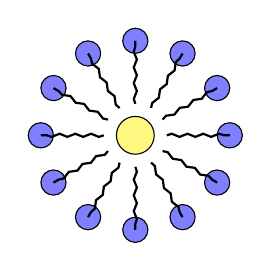
\begin{tikzpicture}[scale=0.8]
    % Draw the hydrophilic heads
    \foreach \angle in {0,30,...,330} {
        \filldraw[fill=blue!50] (\angle:1.5) circle (0.2);
    }
    % Draw the hydrophobic tails as squiggly lines
    \foreach \angle in {0,30,...,330} {
        \draw[thick, decorate, decoration={snake, amplitude=0.2mm, segment length=2mm}] (\angle:0.5) -- (\angle:1.5);
    }
    % Draw the trapped oil in the middle
    \filldraw[fill=yellow!50] (0,0) circle (0.3);
\end{tikzpicture}
\end{center}

\part*{Proteins}

\section*{Station 1}
Suppose that we're using Linda's blood (type A-). 
When anti-A and anti-B antibodies are added to the blood sample, 
the anti-A antibodies will react with the A antigens, 
causing the blood to clump. However, the anti-B antibodies
will not do anything, because there are no B antigens in her 
blood.

\section*{Station 2}
Deer tendons attach the muscle to the bones, allowing for movement. 
They are flexibile but not particularly elastic, allowing the joints
to move but still providing stability. Dog hair helps to keep
the dog warm and protect it from dust and dirt. Porcupine needles are used for 
defense. They are barbed, which makes them difficult to remove.

Collagen forms the deer tendons, keratin forms the dog hair 
and porcupine needles. 

\section*{Station 3}
Each amino acid has the formula, \ch{C_{2}H_{5}O_{2}N}.

The amino acids join together through dehydration synthesis, 
where the OH from the carboxyl group of one amino acid 
and the H from the amino group of another amino acid are removed.
A peptide bond if romed between carbon and nitrogen. 

\section*{Station 4}
The egg albumin dissolves and loses its structure. The process is irreversable 
even if the egg is transfrered to a neutral solution. 
This is because denaturation has occured, which is a process where the protein
unfolds and loses its structure. It is very difficult to 
make the protein refold into its original shape. 

Albumin in chicken eggs stores the amino-acids and proteins for the 
growing embryo. 

\section*{Station 5}
\subsection*{Lab work}
The dog hair, when burnt, smells unpleasant. It differs from the
smell of burning wax and sugar, which smell sweet.

\subsection*{Write up}
The sulfur atoms from cysteine and methionine that 
are released when burning the dog hair might give off the foul smell, as
they are usually associated with decaying matter.


\end{document}